% --- 拉曼实验报告正文 ---

\section{实验目的：}
\begin{enumerate}[label=\arabic* 、, leftmargin=4em, labelsep=0pt]
    \item 了解拉曼散射的基本原理和拉曼光谱的产生机制；
    \item 掌握拉曼光谱仪的基本结构和使用方法；
    \item 学会测量固体和液体样品的拉曼光谱，并对光谱进行初步分析。
\end{enumerate}

\section{实验原理：}

\subsection{拉曼散射的基本原理}

拉曼散射（Raman scattering）是光与物质相互作用的一种非弹性散射过程。当一束单色光照射到样品上时，大部分入射光会发生弹性散射（瑞利散射），即散射光的频率与入射光相同；而极少部分光（约$10^{-6}\sim10^{-8}$）会发生非弹性散射，散射光的频率相对于入射光发生改变，这一现象称为拉曼效应，由印度物理学家C.V.拉曼于1928年首次发现。

从量子力学的观点来看，拉曼散射可以理解为光子与分子振动能级之间的能量交换过程。设入射光子的能量为$h\nu_0$，分子处于基态振动能级$E_0$或激发态振动能级$E_1$。当入射光子与分子相互作用时：

\begin{enumerate}[label=（\arabic*）, leftmargin=4em, labelsep=0pt]
    \item \textbf{瑞利散射}：分子吸收光子后被激发到虚能级，随后返回原来的振动能级，发射出与入射光频率相同的光子（$h\nu_0$）；
    \item \textbf{斯托克斯散射（Stokes scattering）}：分子从基态$E_0$被激发到虚能级后，返回激发态振动能级$E_1$，发射的光子能量为$h(\nu_0 - \nu_m)$，即散射光频率低于入射光频率；
    \item \textbf{反斯托克斯散射（Anti-Stokes scattering）}：分子从激发态$E_1$被激发到虚能级后，返回基态$E_0$，发射的光子能量为$h(\nu_0 + \nu_m)$，即散射光频率高于入射光频率。
\end{enumerate}

% 拉曼散射能级跃迁图
\begin{figure}[htbp]
    \centering
    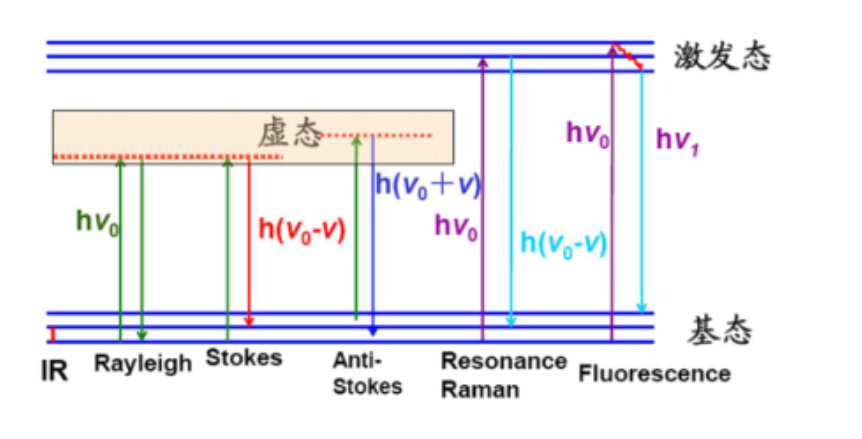
\includegraphics[width=0.55\textwidth]{pictures/能级示意图.png}
    \caption{图1\quad 拉曼散射能级跃迁示意图}
    \label{fig:energy-level}
\end{figure}

拉曼位移（Raman shift）定义为入射光与散射光的波数差：
\begin{equation}
    \Delta\tilde{\nu} = \tilde{\nu}_0 - \tilde{\nu}_s = \frac{1}{\lambda_0} - \frac{1}{\lambda_s}
\end{equation}
其中$\tilde{\nu}_0$和$\tilde{\nu}_s$分别为入射光和散射光的波数（cm$^{-1}$），$\lambda_0$和$\lambda_s$为对应的波长。拉曼位移与入射光波长无关，只取决于分子的振动能级结构，因此拉曼光谱是分子结构的"指纹"。

\subsection{拉曼光谱的特征}

\begin{enumerate}[label=（\arabic*）, leftmargin=4em, labelsep=0pt]
    \item \textbf{斯托克斯线与反斯托克斯线}：在拉曼光谱中，斯托克斯线出现在入射光低频侧（长波长侧），反斯托克斯线出现在高频侧（短波长侧）。由于常温下处于基态的分子数远多于激发态，斯托克斯线的强度通常远大于反斯托克斯线；
    \item \textbf{拉曼位移}：拉曼峰的峰位用拉曼位移（波数差）表示，单位通常为cm$^{-1}$，它与分子特定的振动模式相对应；
    \item \textbf{拉曼活性}：分子的某种振动模式是否具有拉曼活性，取决于振动过程中分子极化率是否发生变化。具有对称中心的分子，红外活性和拉曼活性互相排斥（互斥规则）。
\end{enumerate}

\section{实验仪器：}

本实验使用的主要仪器设备如下：

\begin{enumerate}[label=\arabic* 、, leftmargin=4em, labelsep=0pt]
    \item \textbf{激光器}：波长785nm的半导体激光器，作为激发光源；
    \item \textbf{拉曼探头}：包括入射光纤、收集光纤、滤波片组（瑞利滤光片）和聚焦透镜，用于将激光传输至样品并收集散射光；
    \item \textbf{光谱仪}：用于将收集到的拉曼散射光按波长分散并检测，配有CCD探测器；
    \item \textbf{计算机及软件}：用于控制光谱仪采集数据、显示和处理拉曼光谱。
\end{enumerate}

% 拉曼探头结构图
\begin{figure}[htbp]
    \centering
    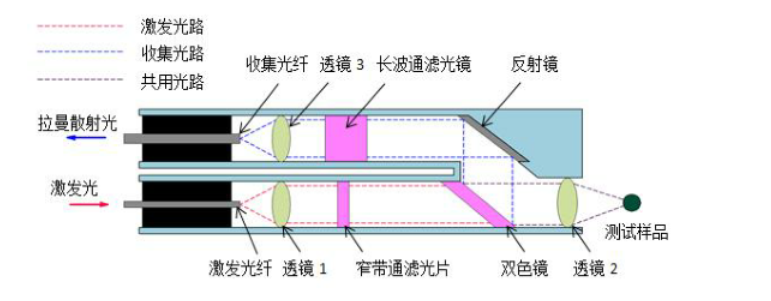
\includegraphics[width=0.6\textwidth]{pictures/探头结构.png}
    \caption{图2\quad 拉曼探头结构示意图}
    \label{fig:probe}
\end{figure}

拉曼探头是拉曼光谱系统的核心部件之一。如图\ref{fig:probe}所示，激光通过入射光纤传输至探头，经带通滤光片滤除杂散光后，由聚焦透镜汇聚到样品表面。样品产生的散射光（包括瑞利散射和拉曼散射）被同一透镜收集，经长通滤光片（或陷波滤光片）滤除瑞利散射光后，通过收集光纤传输至光谱仪进行分光和检测。

\section{实验内容与步骤：}

\subsection{固体样品拉曼光谱测量}

\begin{enumerate}[label=\arabic* 、, leftmargin=4em, labelsep=0pt]
    \item 打开激光器电源，预热约5分钟，使激光输出稳定；
    \item 启动计算机上的光谱采集软件，设置积分时间（如1000ms）、平均次数（如3次）等参数；
    \item 将固体样品（如硅片、A4纸、塑料壳等）放置在样品台上，调整探头位置使激光聚焦于样品表面；
    \item 在软件中设置激光功率（注意避免功率过高损伤样品），开始采集拉曼光谱；
    \item 记录光谱数据，保存谱图文件，标注样品名称和测量条件；
    \item 更换样品，重复上述步骤，完成所有固体样品的测量。
\end{enumerate}

\subsection{液体样品拉曼光谱测量}

\begin{enumerate}[label=\arabic* 、, leftmargin=4em, labelsep=0pt]
    \item 取适量液体样品（如乙醇、丙酮、日落黄溶液、水等）置于石英比色皿中；
    \item 将比色皿放入样品架，调整探头对准比色皿透光面；
    \item 设置合适的积分时间和激光功率，采集拉曼光谱；
    \item 记录光谱数据，保存谱图文件；
    \item 更换液体样品，重复上述步骤；
    \item 测量完毕后，关闭激光器，清理样品和比色皿。
\end{enumerate}

\section{实验数据：}

\subsection{实验条件}

本实验采用 785 nm 半导体激光器作为激发光源，光谱仪型号 HDX01777，CCD 探测器像素数 2068。
各样品测量条件如下表所示：

\begin{table}[htbp]
    \centering
    \caption{各样品拉曼光谱测量条件}
    \label{tab:conditions}
    \begin{tabular}{cccc}
        \hline
        \textbf{样品名称} & \textbf{积分时间 (s)} & \textbf{平均次数} & \textbf{测量时间} \\
        \hline
        黑药片   & 0.8 & 1 & 17:19 \\
        白药片   & 0.8 & 1 & 17:24 \\
        单晶硅   & 0.8 & 1 & 17:28 \\
        无水乙醇 & 0.5 & 1 & 17:45 \\
        \hline
    \end{tabular}
\end{table}

\subsection{拉曼特征峰数据}

各样品经测量得到的拉曼光谱主要特征峰位整理如表~\ref{tab:raman-peaks} 所示。

\begin{table}[htbp]
    \centering
    \caption{各样品拉曼特征峰位汇总（激发波长 785 nm）}
    \label{tab:raman-peaks}
    \begin{tabular}{ccl}
        \hline
        \textbf{样品名称} & \textbf{主要拉曼峰位 (cm$^{-1}$)} & \textbf{归属说明} \\
        \hline
        单晶硅 (Si) & 516.469 & 晶体硅一阶光学声子模（标准值 520.7 cm$^{-1}$）\\
        \hline
        \multirow{6}{*}{无水乙醇 (C$_2$H$_5$OH)} 
            & 880.074 & C—C—O 对称伸缩振动 \\
            & 1048.673 & C—O 伸缩振动 \\
            & 1090.602 & C—O 伸缩振动 \\
            & 1270.61 & CH$_2$ 面外摇摆 \\
            & 1452.094 & CH$_2$ 变形振动（剪式） \\
        \hline
        \multirow{5}{*}{白药片} 
            & 145.029 & 晶格振动或低频骨架弯曲振动 \\
            & 390.673 & 芳环面外变形振动 \\
            & 638.646 & 芳环面内变形振动 \\
        \hline
        \multirow{6}{*}{黑药片} 
            & 209.888 & 晶格振动或分子间振动 \\
            & 328.457 & 骨架弯曲振动 \\
            & 386.553 & 芳环面外变形振动 \\
            & 646.407 & 芳环面内变形振动 \\
        \hline
    \end{tabular}
\end{table}

\section{数据分析：}

根据实验测得的光谱数据，对各样品的拉曼光谱特征进行如下分析：

\subsection{单晶硅 (Si)}

硅片在 516.469 cm$^{-1}$ 处出现尖锐的拉曼特征峰，对应于晶体硅的一阶光学声子模（文献标准值为 520.7 cm$^{-1}$）。
实验测量值与标准值相差约 4.2 cm$^{-1}$（相对误差约 0.8\%），该偏差在光谱仪波数校准误差的允许范围内。
该峰形对称、半高宽很窄（约 4--5 cm$^{-1}$），表明所测硅片具有良好的晶体质量。
硅的一阶光学声子峰是拉曼光谱仪最常用的波数校准标准峰之一。

\subsection{无水乙醇 (C$_2$H$_5$OH)}

乙醇的拉曼光谱呈现出丰富的振动特征峰，反映了乙醇分子中各官能团的振动模式：
\begin{enumerate}[label=(\arabic*), leftmargin=3em]
    \item \textbf{C—C—O 骨架振动区（880.074 cm$^{-1}$）：} 该峰为乙醇的最强拉曼峰，归属为 C—C—O 的对称伸缩振动，是乙醇分子骨架的特征谱带；
    \item \textbf{C—O 伸缩振动区（1048.673 cm$^{-1}$、1090.602 cm$^{-1}$）：} 这两个峰对应于 C—O 键的伸缩振动，其中 1048.673 cm$^{-1}$ 峰对应于反式构象，1090.602 cm$^{-1}$ 峰对应于邻位交叉构象；
    \item \textbf{CH$_2$ 变形振动区（1270.61 cm$^{-1}$、1452.094 cm$^{-1}$）：} 1270.61 cm$^{-1}$ 归属为 CH$_2$ 面外摇摆振动，1452.094 cm$^{-1}$ 为 CH$_2$ 剪式变形振动。
\end{enumerate}

\noindent 所有观察到的拉曼峰与文献报道的乙醇拉曼光谱数据吻合良好，验证了拉曼光谱作为分子结构"指纹"的可靠性。

\subsection{白药片与黑药片}

对比白药片与黑药片的拉曼光谱，两者在低波数区（100--650 cm$^{-1}$）均表现出若干特征峰，但峰位和峰数存在明显差异：
\begin{itemize}
    \item 白药片在 145.029 cm$^{-1}$、390.673 cm$^{-1}$ 和 638.646 cm$^{-1}$ 处出现三个主要拉曼峰。其中 145 cm$^{-1}$ 附近的低波数峰通常对应于分子间弱相互作用或晶格振动模式，390 cm$^{-1}$ 和 639 cm$^{-1}$ 处的峰可能归属于芳环的面外和面内变形振动，表明白药片中含有芳香族化合物成分；
    \item 黑药片在 209.888 cm$^{-1}$、328.457 cm$^{-1}$、386.553 cm$^{-1}$ 和 646.407 cm$^{-1}$ 处出现四个主要拉曼峰。与白药片相比，黑药片在 200--330 cm$^{-1}$ 范围内多出两个低波数峰，且 387 cm$^{-1}$ 附近的峰位与白药片接近但强度可能有所不同，646 cm$^{-1}$ 附近的峰位两者基本一致，说明两种药片可能含有相同的芳香骨架结构；
    \item 两种药片在 640 cm$^{-1}$ 附近的峰位接近，提示它们可能共享相同或相似的活性成分。黑药片多出的低波数峰（209 cm$^{-1}$ 和 328 cm$^{-1}$）可能来源于辅料成分（如淀粉、硬脂酸镁或其他赋形剂）的特征振动；
    \item 白药片与黑药片的拉曼峰均集中在低波数区（< 650 cm$^{-1}$），在高波数区未观察到显著的 C—H、C=O 或 O—H 伸缩振动峰，这可能是由于样品本身对这些振动模式的拉曼散射截面较小，或实验条件（积分时间较短）导致高波数区信号较弱。
\end{itemize}

\noindent 综上，白药片和黑药片在低波数区的拉曼峰差异为两者的鉴别提供了依据。通过对比特征峰的数目和位置，拉曼光谱能够快速、无损地区分外观相似但组成不同的药物制剂，在药品快速筛查和质量控制中具有潜在的应用价值。

\subsection{总体讨论}

\begin{enumerate}[label=\arabic* 、, leftmargin=4em, labelsep=0pt]
    \item 实验成功测量了四种样品的拉曼光谱，各样品在低波数区特征峰清晰可辨；
    \item 硅的一阶声子峰（516.469 cm$^{-1}$）可作为波数校准参考，与标准值（520.7 cm$^{-1}$）偏差较小；
    \item 乙醇光谱与标准谱库吻合良好，验证了实验系统的可靠性；
    \item 白药片和黑药片在低波数区呈现不同的拉曼峰特征，峰位和峰数的差异为两者的快速鉴别提供了依据；
    \item 拉曼光谱技术具有快速、无损、无需样品前处理等优点，特别适用于药物、化工、材料等领域的定性分析。
\end{enumerate}

\section{思考题：}

\begin{enumerate}[label=\arabic* 、, leftmargin=4em, labelsep=0pt]
    \item \textbf{什么是斯托克斯散射和反斯托克斯散射？为什么常温下斯托克斯线强度远大于反斯托克斯线？} \\
    答：斯托克斯散射是指散射光子能量低于入射光子能量的拉曼散射过程，此时分子从基态振动能级被激发后返回较高的振动能级；反斯托克斯散射是指散射光子能量高于入射光子能量的过程，此时分子从激发态振动能级被激发后返回基态。根据玻尔兹曼分布定律，常温下处于振动基态的分子数远多于激发态的分子数，因此发生斯托克斯散射的概率远大于反斯托克斯散射，导致斯托克斯线强度远大于反斯托克斯线。

    \item \textbf{如何选择拉曼光谱的激发波长？785nm激光相对于532nm激光有何优缺点？} \\
    答：选择激发波长时需要综合考虑荧光干扰、信号强度和检测器响应等因素。
    785nm激光的优点：（1）光子能量较低，能有效减少样品荧光背景的干扰，尤其适合有机样品和生物样品的测量；（2）对样品的损伤较小。缺点：（1）拉曼散射强度与$\lambda^{-4}$成正比，长波长激光的拉曼信号较弱；（2）CCD探测器在近红外区的量子效率较低。
    532nm激光的优点：拉曼信号强度大，探测器效率高。缺点：容易激发出强的荧光背景，干扰拉曼信号的检测。因此对于易产生荧光的样品（如有机物、生物样品），优先选用785nm或更长波长的激光；对于荧光较弱的无机样品，可选用532nm激光以获得更高的灵敏度。

    \item \textbf{拉曼位移的波数(cm$^{-1}$)与波长(nm)、频率(Hz)以及能量(eV)之间如何换算？} \\
    答：各物理量之间的换算关系如下：
    \begin{itemize}
        \item 波数$\tilde{\nu}$ (cm$^{-1}$) 与波长$\lambda$ (nm) 的关系：$\tilde{\nu} = \frac{10^7}{\lambda}$
        \item 频率$\nu$ (Hz) 与波长$\lambda$ (nm) 的关系：$\nu = \frac{c}{\lambda} = \frac{3\times10^{17}}{\lambda}$
        \item 能量$E$ (eV) 与波长$\lambda$ (nm) 的关系：$E = \frac{hc}{\lambda} = \frac{1240}{\lambda}$
        \item 波数$\tilde{\nu}$ (cm$^{-1}$) 与能量$E$ (eV) 的关系：$E = hc\tilde{\nu} \approx 1.24\times10^{-4}\,\tilde{\nu}$
    \end{itemize}
    拉曼位移表示的是入射光与散射光的波数差，即$\Delta\tilde{\nu} = \tilde{\nu}_0 - \tilde{\nu}_s$，它直接反映分子振动能级间的能量差。
\end{enumerate}
